

\chapter{Konstruktion und Design}
\label{chap:konstruktion}
\section{Wahl des Bootstypus}
\subsection{Vergleich von verschiedenen Segelboot Typen - Entschiedbaum}
\subsubsection{Rumpftypen}
Die erste und einfachste Unterscheidung von verschiedenen Segelboot Typen ist die Anzahl an Rümpfen. Wenn man sich ein Segelboot vorstellt, denkt man meist an ein ”mono hull”. Jedoch gibt es auch den ”double hull¨ der man Kategorisiert sie als ”multi hull”, welche vorallem aus der Welt der Ka- thamarane und Trimarane bekannt sind.
Der Rumpf an sich kann jedoch auch innerhalb von einer von diesen Kategorien komplett unterschiedlich geformt sein.
Kielboote vs. Jollen

\subsubsection{Segeltypen}
\subsubsection{Kieltypen}
 \subsubection{Rudertypen???}
\section{Entscheid für ein Kielboot}
\subsection{Entscheid für eine Eigenentwicklung}

\section{Strukturelles Design des autonomen Segelschiffs}



%->	Baupläne werden generiert als Resultat
\subsection{Vergleich von verschiedenen Segelboot Typen}

\subsubsection{Rumpftypen}
Die erste und einfachste Unterscheidung von verschiedenen Segelboot Typen ist die Anzahl an Rümpfen. Wenn man sich ein Segelboot vorstellt, denkt man meist an ein "mono hull". Jedoch gibt es auch den "double hull" oder man Kategorisiert sie als "multi hull" welche vorallem aus der Welt der Kathamarane und Trimarane bekannt sind.\\
Der Rumpf an sich kann jedoch auch innerhalb von einer von diesen Kategorien komplett unterschiedlich geformt sein. 
%
\subsubsection{Segeltypen}

\subsubsection{Kieltypen}

\subsubsection{Rudertypen}


\section{Materialauswahl und -begründung }
% Turn around 

Die strukturell Tragenden Elemente sind Hauptsächlich aus Holz gebaut. Dies hat den entscheidenden Vorteil der einfachen Verarbeitung. Ebenso hat Holz den Vorteil, dass es an sich schon schwimmt da es weniger Dicht als Wasser ist. Konkret werden zwei Holzarten verwedet. Zum einen Tannenholz und zum anderen Balasaholz. Das Tannenleimholz wird mit einer Stärke von 18mm verbaut und ist das kostengünstigste Holz was in dieser Kategorie im Baumarkt zu finden ist.
Alternativen zu Holz wären diverse Kunststoffe wie PLA, ABS, PETG, ect. welches durch 3D Druck geformt werden können. Jedoch wären die Kosten bei dieser Methode deutlich höher und eine gleiche Stabilität wie bei Holz zu erreichen wäre eine Herausforderung.
Ebenfalls möglich sind Rippenelemente aus Metallen, wie zum Beispiel Aluminium. Die Materialkosten sind bei Metallen jedoch weitaus höher und die Bearbeitung um ein vielfaches Komplizierter weshalb sich dagegen entschieden wurde.
\\
Fu¨ r die Beplankung wird Balsaholz verwendet, da dieses sehr weich, biegsam und einfach zu be- und verarbeiten ist. Es ist im Modellbau weit verbreietet und in diversen Stärken verfügbar. In geringen Stärken von 1mm laässt es sich gut an die Form des Bootes anpassen.
% Balsaholz ABschnitt hinzufügen

\subsection{Fiberglas}
Da Balsaholz sehr porös ist, darf es unbehandelt nicht Wasser ausgesetzt werden. Selbst wenn es mit Lack gegen Feuchtigkeit geschützt wird, ist eine Balsaholzuhülle zu wenig robust, um die Aussenhülle des Bootes zu bilden.

Für die äussere Hülle werden Fiberglasmatten verwendet. Diese sorgen für eine stabile Hülle und schützen das Boot zusätzlich vor seitlichen Zusammenstössen. Ebenfalls sorgen sie dafür, dass das Boot dicht ist und kein Wasser hineinfliesst. Alternativ hätte man das Boot lediglich mit Epoxidharz abdichten können. Dies hätte aber dazu geführt, dass das Boot um ein vielfaches weniger stabil wäre. 

\section{Prozess der Konstruktion}
Bei der Konstruktion geht es um die Erstellung von Plänen. Das erfolgt bei komplexeren Konstruktionen immer computergestützt mittels sogenannten \ac{cad} Programmen. 

\subsection{Applikation}
Computer Aided Design (CAD) ist eine Form des technischen Zeichens, welches einem ermöglicht Modelle in Drei dimensionalen Raum zu gestalten. Somit lässt ist es verhältnissmässig einfach Technische Zeichnungen anzufertigen. Es gilt als eines der Wichtigsten Werkzeuge zur Planung von Maschienen und Geräten da sie so einfacher Vorstellbar sind und der Materialbedarf geplant werden kann. Die Konstruktion dieses Projekt beginnt mit dem erlernen von den Programmen Autodesk Inventor und Autodesk Fusion 360. 
Beide Programme verfolgen einen ähnlichen Ansatz und sind ähnlich Aufgebaut. Im Vergleich zu Inventor ist Fusion deutlich nutzerfreundlicher und ermöglicht es Projekte über eine Cloud einfacher zu speichern und von Unterwegs zu Bearbeiten. Die Programme von Autodesk wurden gewählt, da diese für den Persönlichen oder Bildungsgebrauch kostenlos sind. Open Source Programme wie FreeCAD wurden nicht gewählt, da diese weniger Intuitiv zum lernen sind und meist über weniger Funktionen verfügen. Programme welche als deutlich Leistungsstarker gelten wie NX Siemens oder Solidworks sind aufgrund der Lizensierungskosten für dieses Projekt nicht in Frage gekommen. 

\subsection{Konstruktionsvorgang des Rumpfes}
Da eine ebene Fläche für die Positionierung der Solarpanels benötigt wird, wird das Deck flach ausgelegt. Es bildet den Ausgangspunkt des Entwurfs. In einer Skizze wird die spätere Bootsform mithilfe gezeichnet. Da das Boot Wellen und Wetterbeständig sein sollte, muss das Boot über genügend Auftrieb verfügen. Daher wird eine Länge von 2.2m gewählt. \\
Für die maximale Breite werden 0.55m verwendet. Dies entspricht einem Viertel der Länge. Das Verhältnis zwischen der Länge und der Breite ist der Einflussreichste Faktor welcher über  Stabilität und die Manövrierfähigkeit. Ein Verhältnismässig Breites Boot ist deutlich stabiler als ein schmaleres, jedoch weniger Manövrierfähig. \cite{Seemannschaft} \\
\begin{figure}[H]
    \centering
    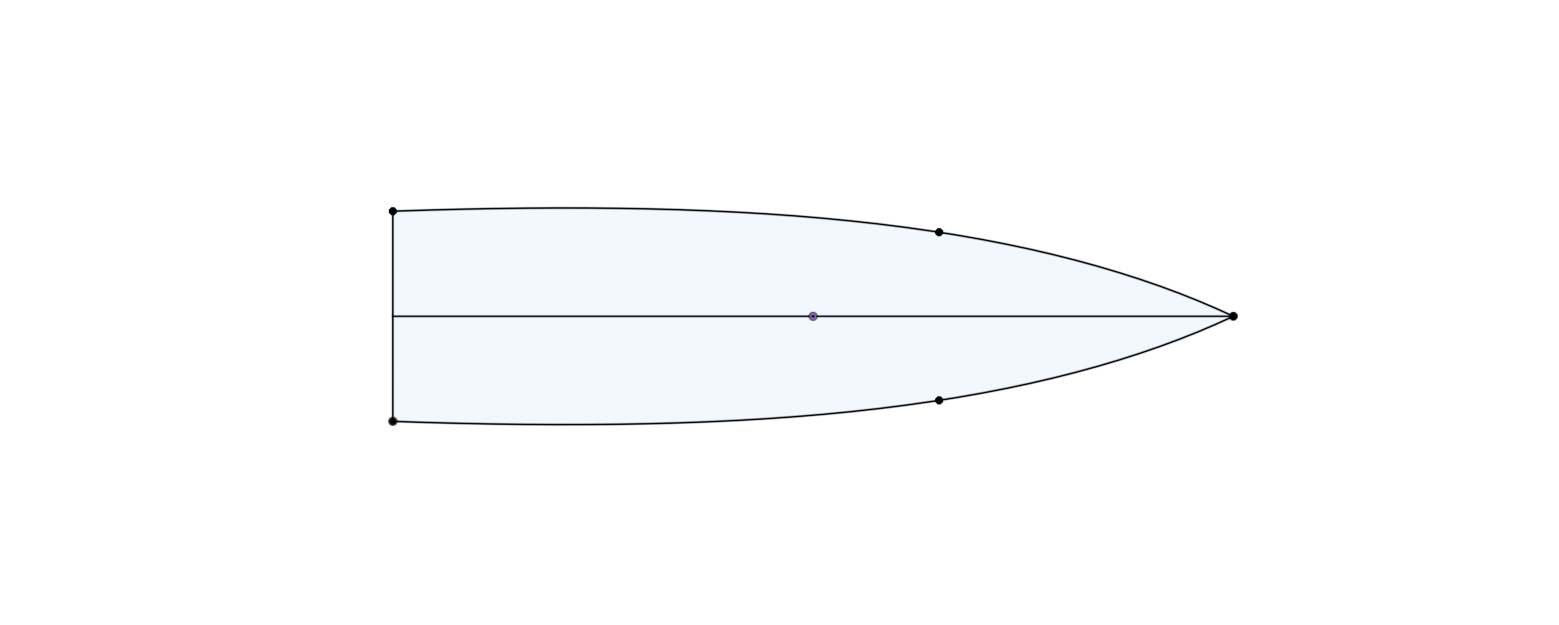
\includegraphics[width=1\linewidth]{assets/boot sketch top.png}
    \caption{Topansicht des Boots}
   
\end{figure}
In einem nächsten Schritt wird die Seitenansicht des Bootes konstruiert. Dieses Boot verfügt über einen angewinkelten Vorsteven und ein flaches Heck. Das Flache Heck wird gewählt, da die Befestigung des Ruders so am einfachsten ist und der Bug nach Hinten angewinkelt.

\begin{figure}[H]
    \centering
    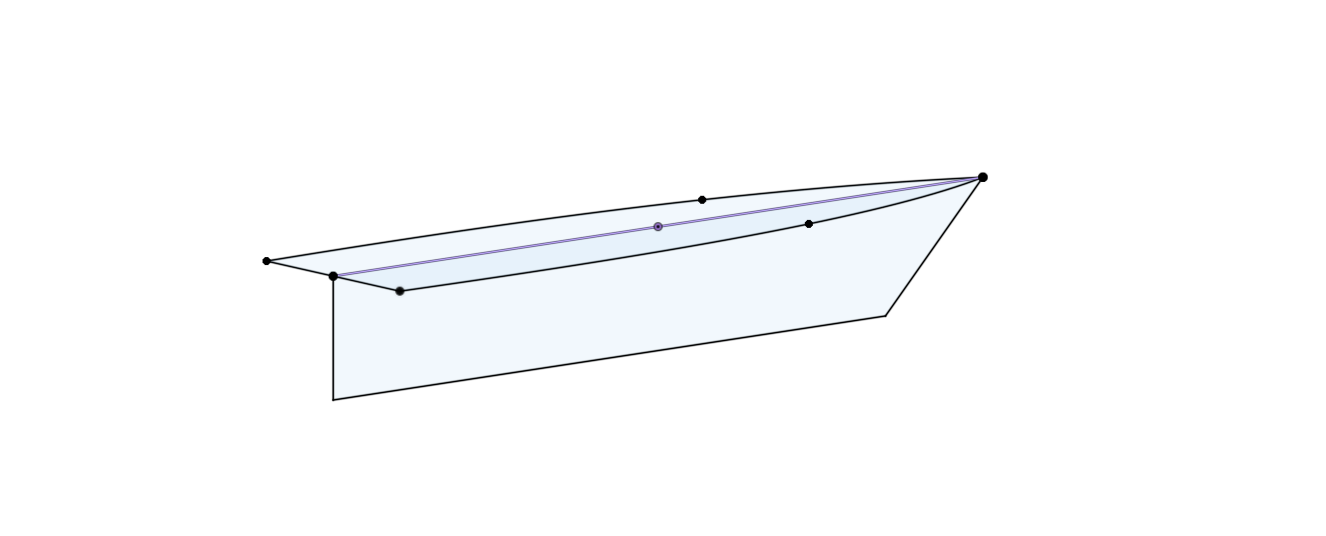
\includegraphics[width=1\linewidth]{assets/boot_skizze_2.png}
    \caption{Seitenansicht mit Steven}
    
\end{figure}

Als Heckform wurde eine leicht eingebeulte Form verwendet, welche dem Boot verhilft, senkrecht im Wasser zu stehen.

\begin{figure}[H]
    \centering
    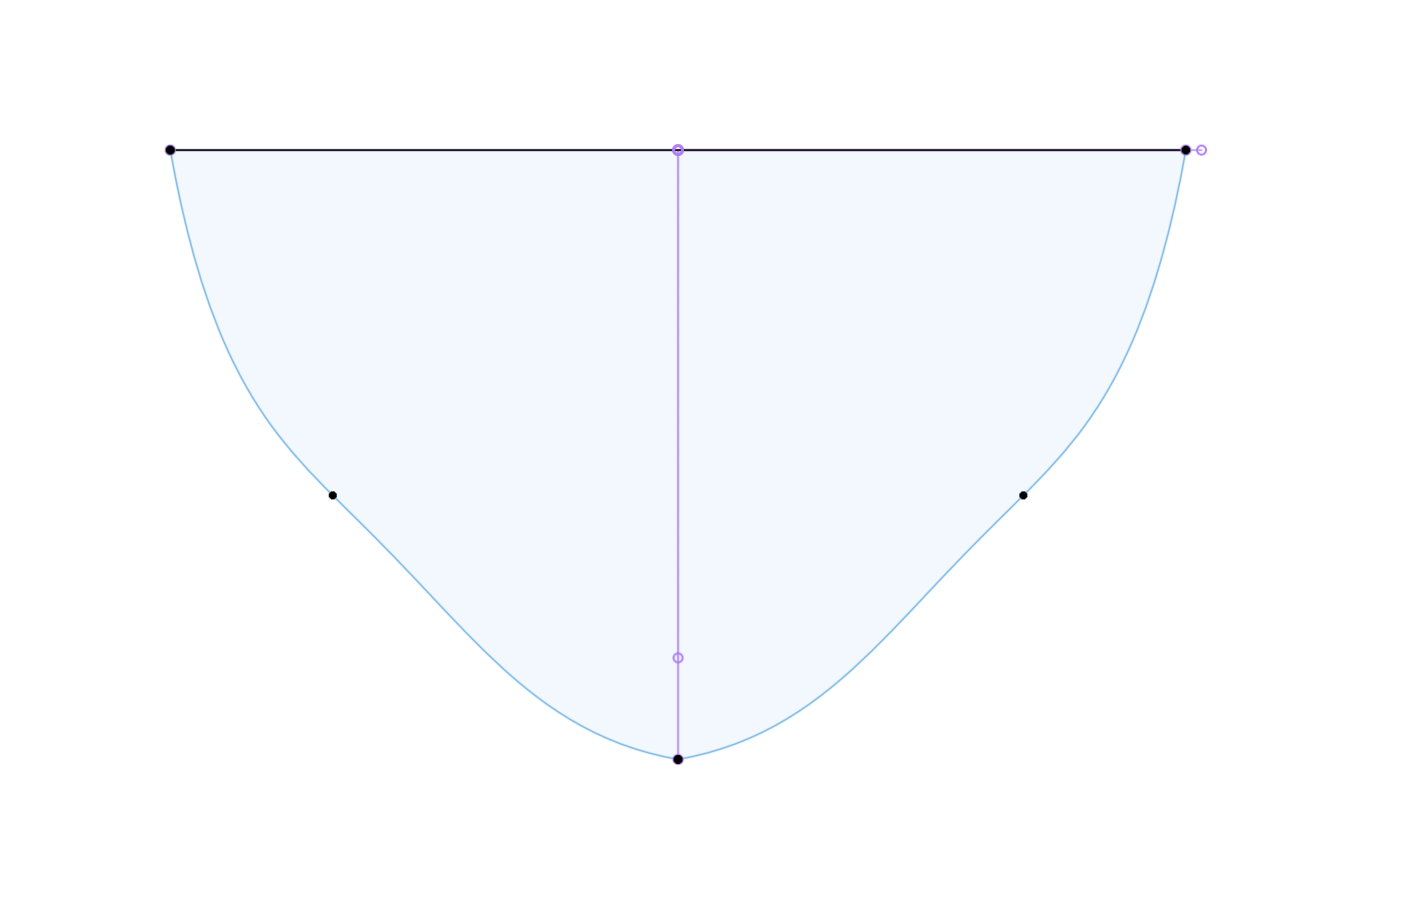
\includegraphics[width=0.6\linewidth]{assets/Heck_boot.png}
    \caption{Heckansicht}
   
\end{figure}

Mit dem Erhebungswerkzeug (Loft Tool) wird im Anschluss aus den Skizzen ein Körper berechnet. Unten am Rumpf wird zudem eine Begradigung hinzugefügt welche es ermöglicht den Kiel senkrecht am Boot zu montieren.
\begin{figure}[H]
    \centering
    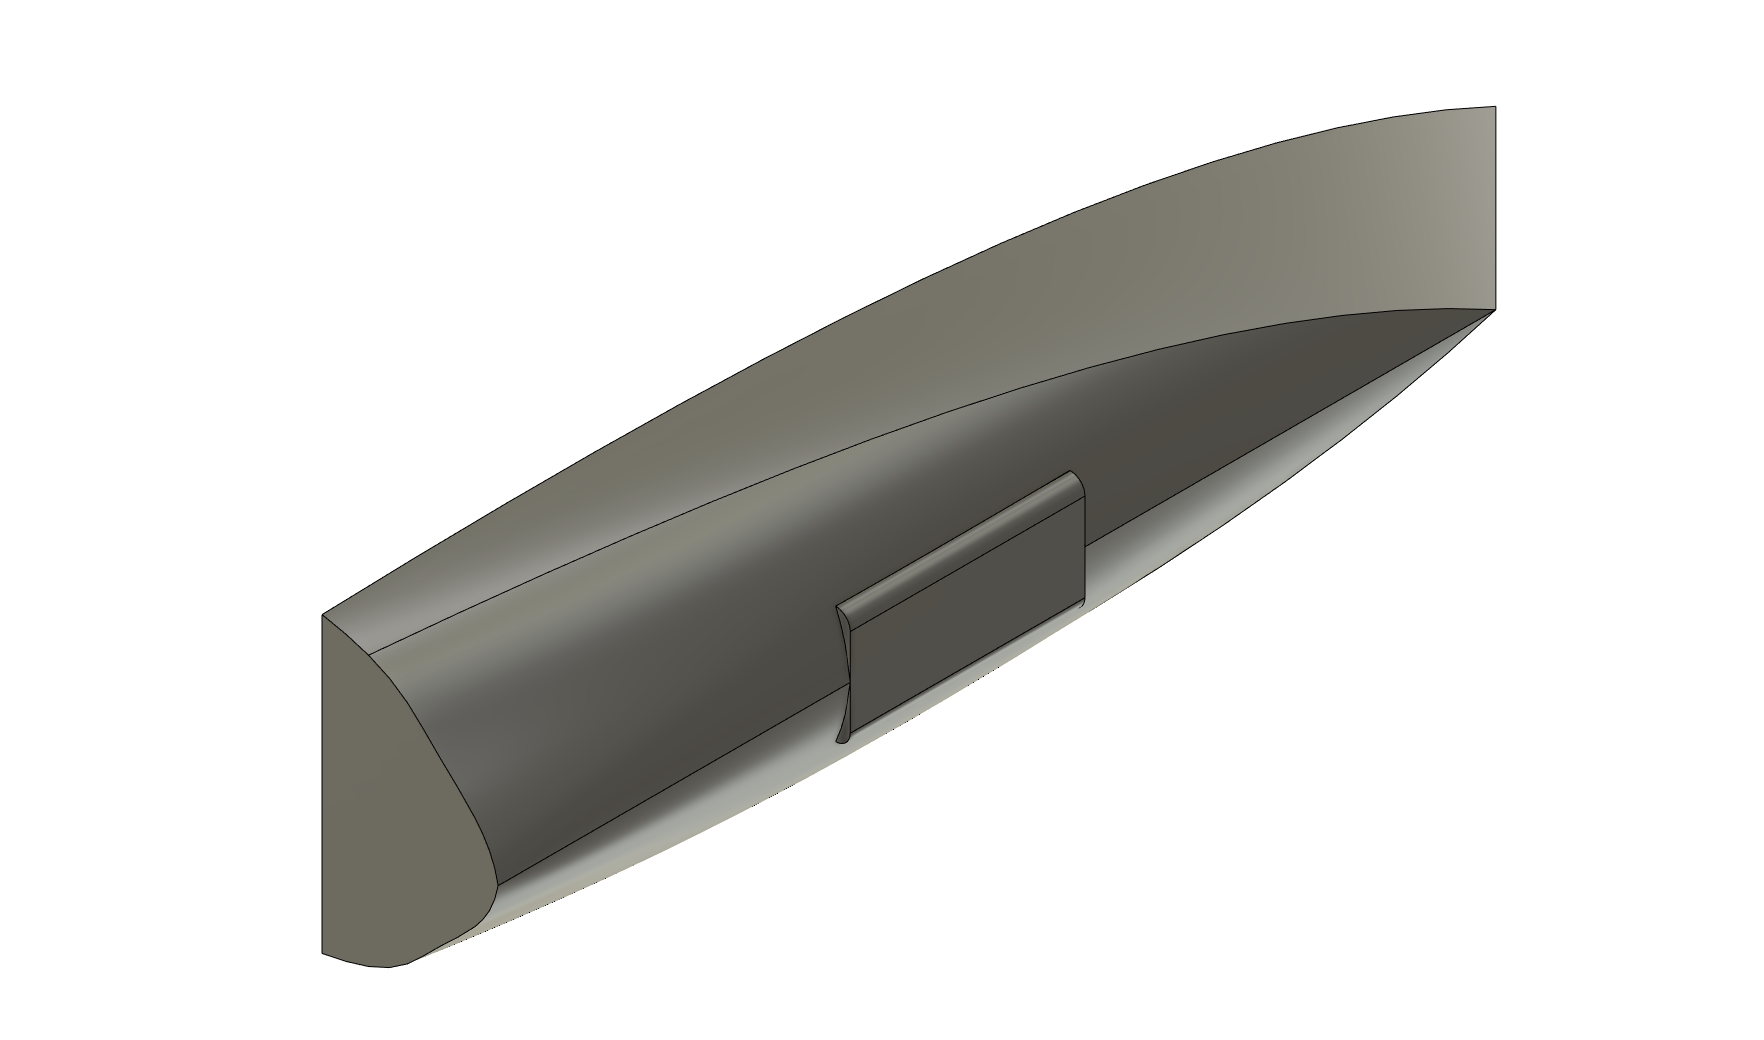
\includegraphics[width=0.75\linewidth]{assets/kielbefestigung2image.png}
    \caption{Fläche zur Montierung es Kiels}
    \label{fig:enter-label}
\end{figure}

Im Anschluss wird die Form mit einer Randstärke von 4 cm innen ausgehölt. 
\begin{figure}[H]
    \centering
    \includegraphics[width=1\linewidth]{assets/Hohlkörper.png}
    \caption{Schnittbild Hohlkörper}

\end{figure}
Im nächsten Schritt wird der bereits ausgehöhlte Körper auf zwölf Spanten mit einem einheitlichem Abstand 14 cm reduziert. Die Spanten haben eine Stärke von 18 mm. 

\begin{figure}[H]
    \centering
    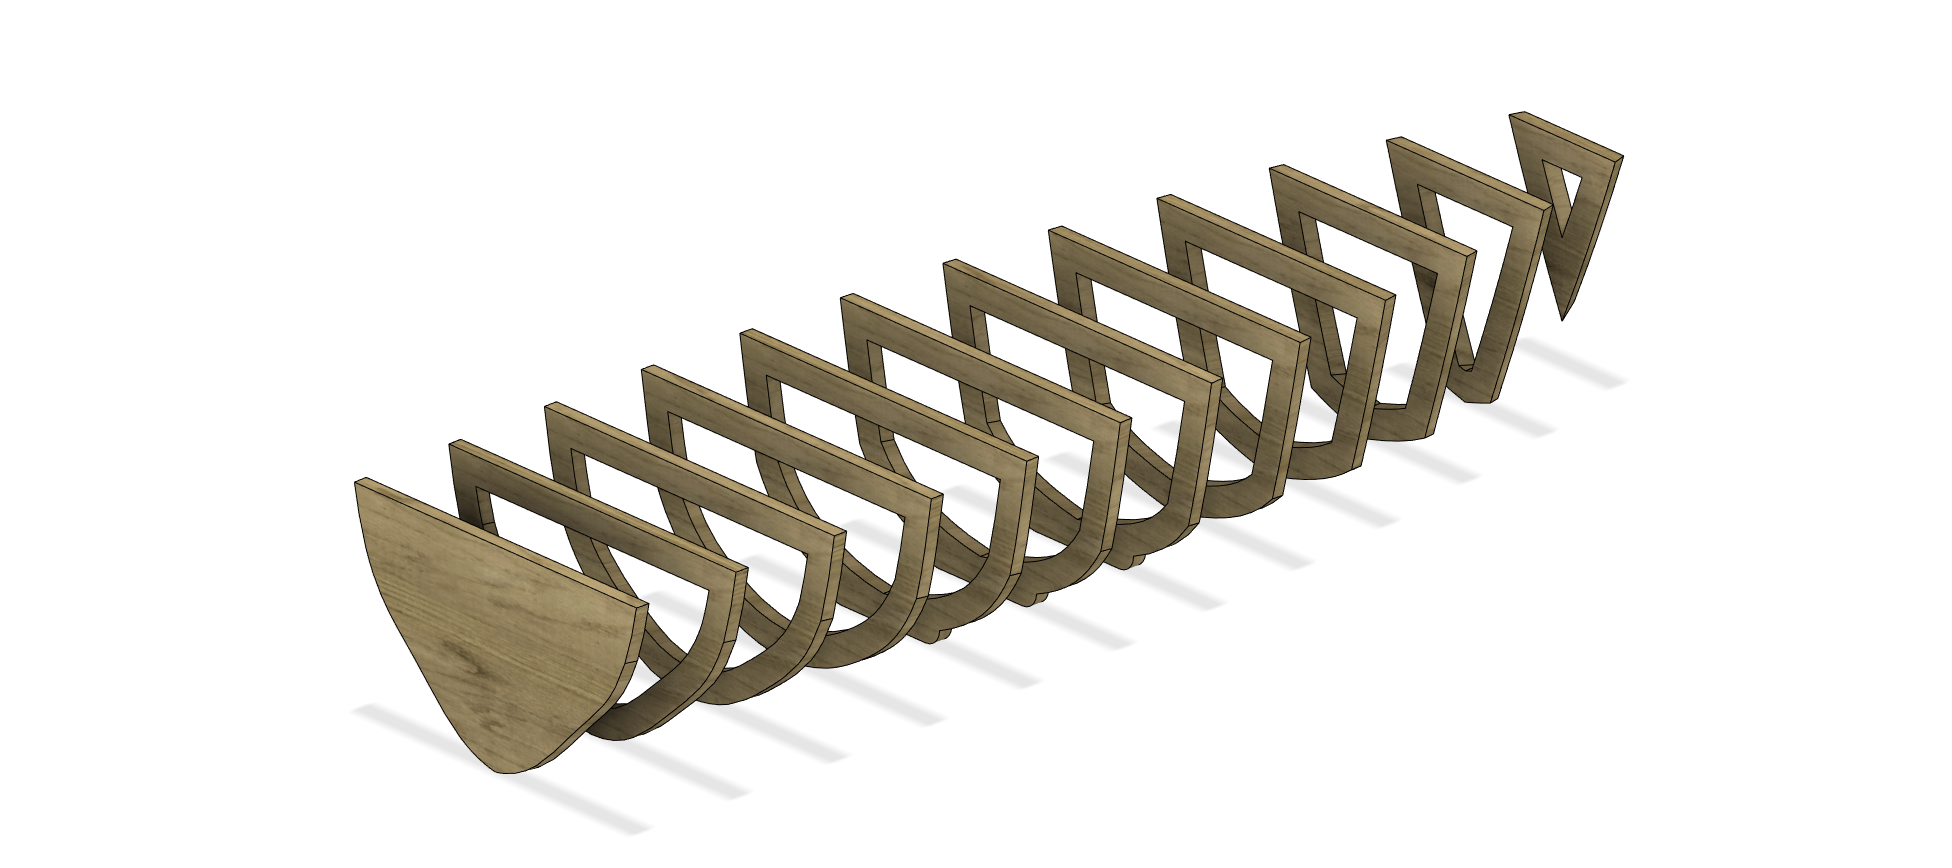
\includegraphics[width=1\linewidth]{assets/rippen_cad.png}
    \caption{Spantenansicht}
    
\end{figure}
Die letzte Spannte ist nicht hohl, weil sie sich am Ende des Hohlkörpers befindet.  \\
Da der Bug des Bootes spitz zu läuft, wurde auf eine Frontspannte verzichtet. Da die Form der Spitze in Holz schwierig umzusetzen ist, wird diese nicht aus Holz sondern als ganzes im 3D Druckverfahren erstellt.
\begin{figure}[H]
    \centering
    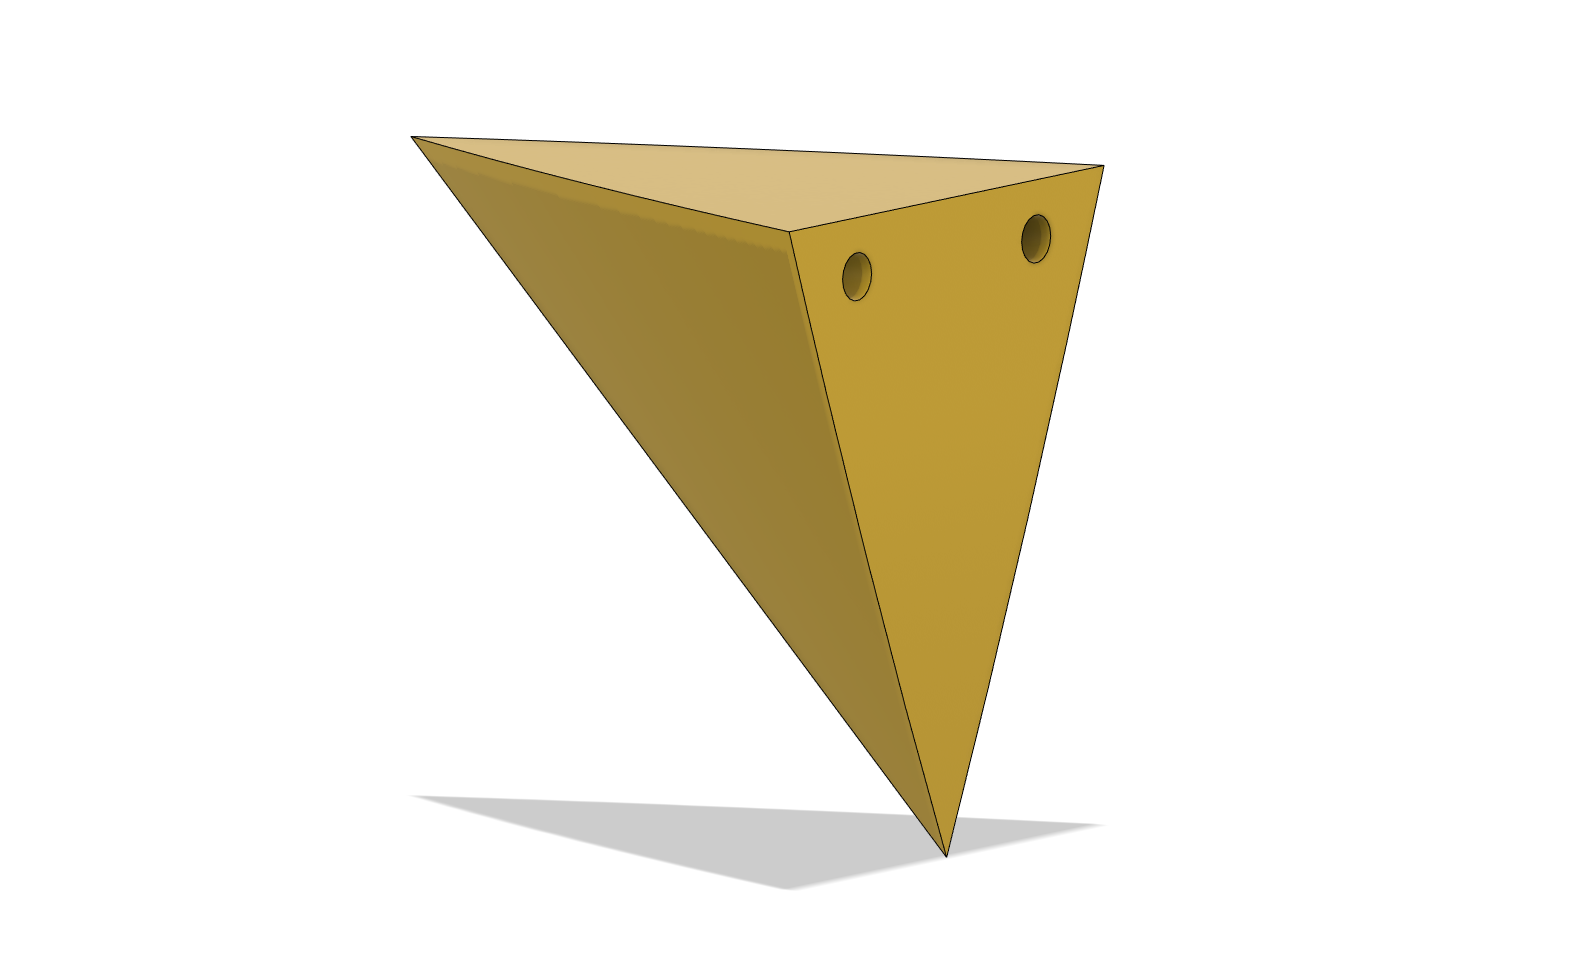
\includegraphics[width=0.8\linewidth]{assets/bug_spitz.png}
 \caption{Bug Spitz}
    
\end{figure}

Um die Spanten untereinander zu verbinden sind zwei Allumniumrohre mit einem Durchmesser von 16 mm vorgesehen. Dafür werden im oberen Holm der Spanten zwei runde Löcher im Abstand von 10 cm geplant. Im Spitz sind diese als Hohlöffnungen vorgesehen. 



\begin{figure}
    \centering
    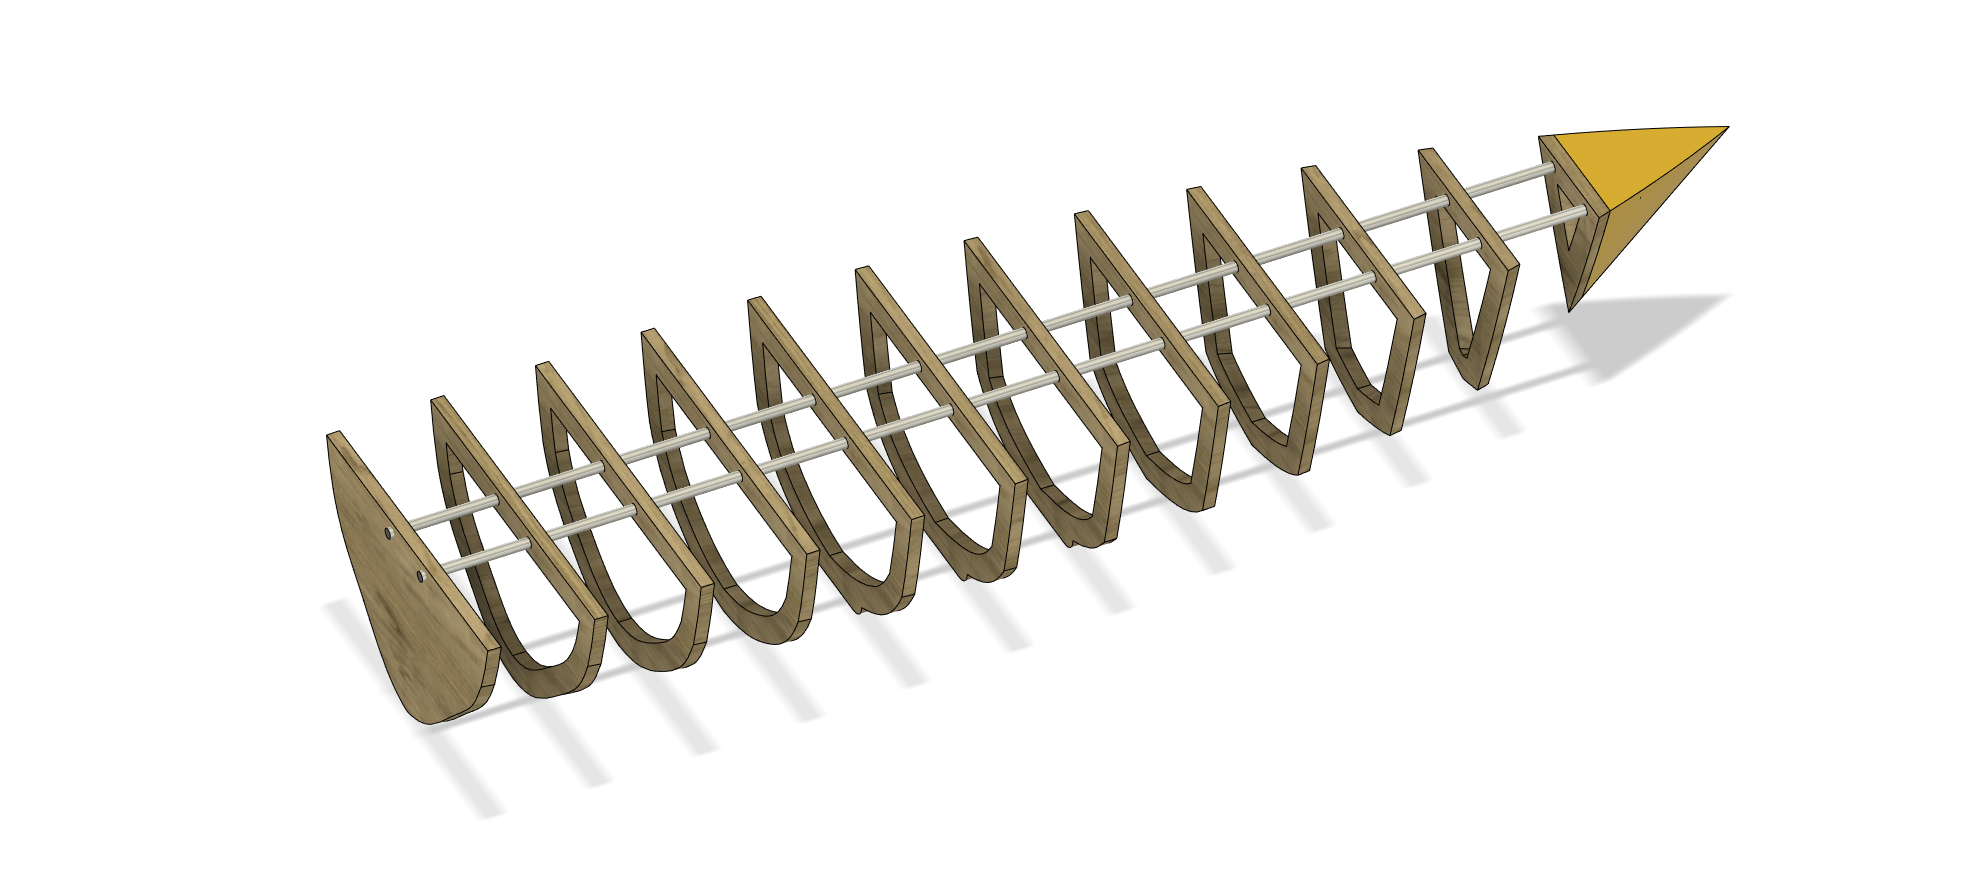
\includegraphics[width=1\linewidth]{assets/full_skellet.png}
    \caption{Abbild der Spanten und des Spitzes in Verbindung}
    
\end{figure}

%\begin{figure}[H]
%  \centering
%  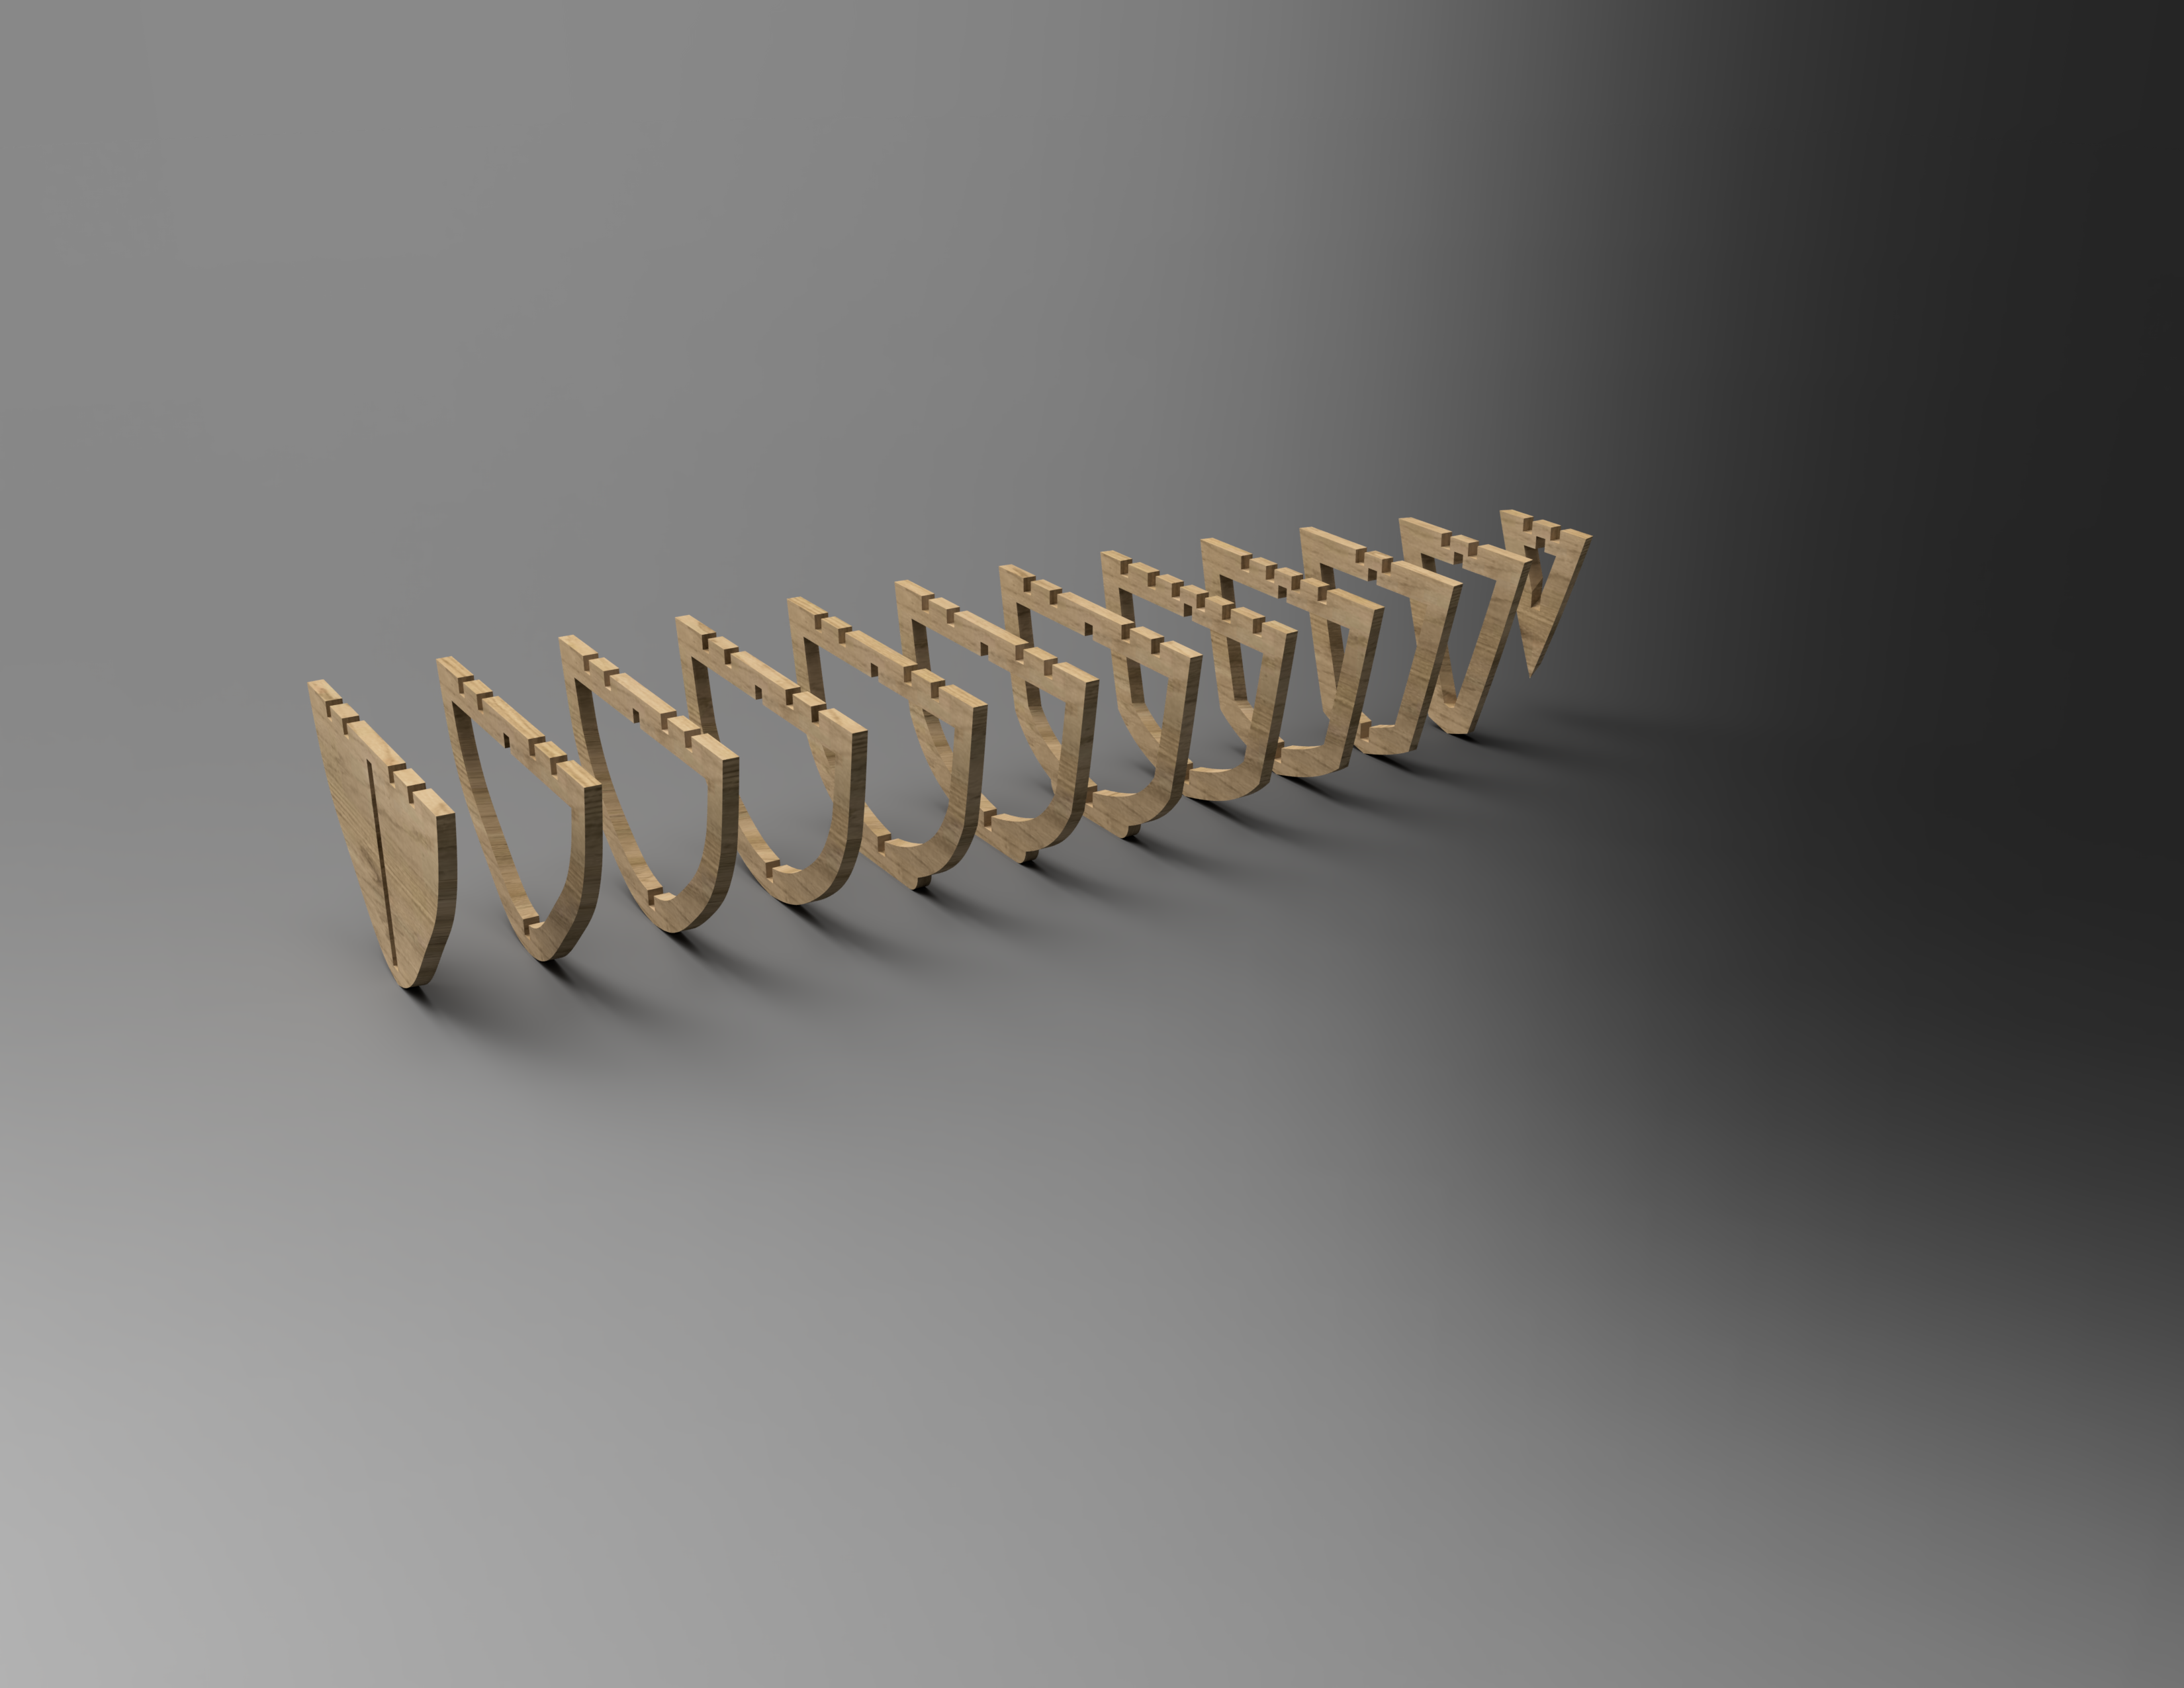
\includegraphics[width=\textwidth]{assets/rippenv1.png}
%  \caption{Render einer ersten Version des Rippenmusters (nicht Final) }
%  \label{fig:rippenv1}
%\end{figure}




\section{Segel und Sailflap}
Beim Design des Segels wurde viel von einer Bestehenden Arbeit übernommen. Diese hat sich mit der Entwicklung eines Segels für den Einsatz auf dem Baltischen Meer spezialisiert.



\section{Entwicklungsprozess des Kiels}
Der Entwicklungsprozess des Kiels ist aufgrund der geringen Literatur in diesem Bereich sehr aufwendig. \\ Die erste Frabstellung in diesem Bereich, ist ob es sich um ein Kiel oder ein Schwert handeln soll. Die Unterschiedung liegt grob darin, dass ein Kiel zusätzliches Gewicht trägt, um das Boot aufrechter zu halten und Schwerter lediglich den Wasserwiederstand. Kiele sind hauptsächlich aus der Welt der Jachten bekannt und Schwerter aus der Welt der Jollen. \\
Für dieses Boot wurde sich für ein Kiel entschieden, da es auf dem Boot keine möglichkeit gibt, Gewicht zu verschieben. Bei Jollen ist in der regel ein Segler auf dem Boot, welcher sehr viel mit seinem eigenen Körpergewicht steuert. Bei den meisten Jachten spielt das Körpergewicht der Segler keine oder nur eine untergeordnete Rolle.